\documentclass[tikz,border=4pt]{standalone}
\usepackage[T1]{fontenc}
\usepackage{lmodern}
\usepackage{amsmath}
% Shared TikZ style for the report figures.
% Colours follow the Okabe-Ito palette, which stays distinguishable under the
% common forms of colour-vision deficiency. Every colour-coded element also
% carries a text label, so no figure depends on colour alone.
\usetikzlibrary{arrows.meta,positioning,fit,calc,backgrounds,decorations.pathreplacing,shapes.geometric}

\definecolor{oiOrange}{HTML}{E69F00}
\definecolor{oiSky}{HTML}{56B4E9}
\definecolor{oiGreen}{HTML}{009E73}
\definecolor{oiYellow}{HTML}{F0E442}
\definecolor{oiBlue}{HTML}{0072B2}
\definecolor{oiVerm}{HTML}{D55E00}
\definecolor{oiPurple}{HTML}{CC79A7}
\definecolor{oiGray}{HTML}{6E6E6E}

\colorlet{corTreino}{oiBlue!22}
\colorlet{corValid}{oiGreen!30}
\colorlet{corTeste}{oiOrange!45}
\colorlet{corControle}{oiPurple!35}

\tikzset{
  >=Stealth,
  bloco/.style={draw=black!70, rounded corners=1.5pt, minimum height=0.62cm,
    inner sep=2pt, font=\sffamily\fsz, align=center},
  treino/.style={bloco, fill=corTreino},
  valid/.style={bloco, fill=corValid},
  teste/.style={bloco, fill=corTeste, thick},
  etapa/.style={draw=black!70, rounded corners=3pt, fill=black!4,
    text width=4.3cm, align=center, inner sep=4pt, font=\sffamily\fsz},
  nota/.style={font=\sffamily\fsz, align=left, text=black!80},
  titulo/.style={font=\sffamily\fst\bfseries, anchor=west},
  seta/.style={->, thick, black!70},
  regiao/.style={draw=black!50, dashed, rounded corners=4pt},
}

% Absolute font sizes, so a figure looks the same standalone (10 pt class) and
% inside the 11 pt report.
\providecommand{\fsx}{\fontsize{5.5}{6.5}\selectfont}
\providecommand{\fsz}{\fontsize{7}{8.5}\selectfont}
\providecommand{\fst}{\fontsize{9}{11}\selectfont}

\begin{document}
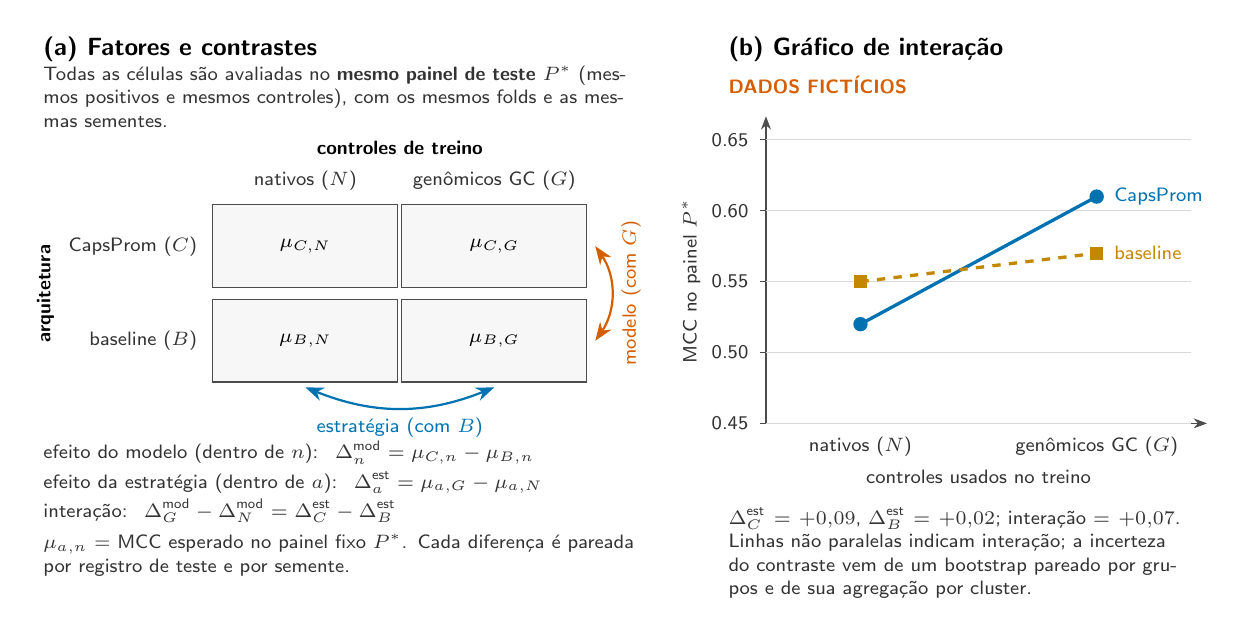
\begin{tikzpicture}[
  celula/.style={draw=black!70, minimum width=2.7cm, minimum height=1.05cm, align=center, font=\sffamily\fsz, fill=black!3},
  efeito/.style={<->, thick},
  ]
  % ---------------- (a) factorial grid ----------------
  \node[titulo] at (0,1.55) {(a) Fatores e contrastes};
  \node[nota, anchor=west, text width=7.6cm] at (0,0.95)
    {Todas as células são avaliadas no \textbf{mesmo painel de teste} $P^\ast$ (mesmos positivos e mesmos controles), com os mesmos folds e as mesmas sementes.};
  \node[font=\sffamily\fsz\bfseries] at (4.65,0.3) {controles de treino};
  \node[nota] at (3.45,-0.12) {nativos ($N$)};
  \node[nota] at (5.85,-0.12) {genômicos GC ($G$)};
  \node[font=\sffamily\fsz\bfseries, rotate=90] at (0.15,-1.55) {arquitetura};
  \node[nota, anchor=east] at (2.2,-0.95) {CapsProm ($C$)};
  \node[nota, anchor=east] at (2.2,-2.15) {baseline ($B$)};
  \node[celula, minimum width=2.35cm] (CN) at (3.45,-0.95) {$\mu_{C,N}$};
  \node[celula, minimum width=2.35cm] (CG) at (5.85,-0.95) {$\mu_{C,G}$};
  \node[celula, minimum width=2.35cm] (BN) at (3.45,-2.15) {$\mu_{B,N}$};
  \node[celula, minimum width=2.35cm] (BG) at (5.85,-2.15) {$\mu_{B,G}$};
  \draw[efeito, oiBlue] ($(BN.south)+(0,-0.06)$) to[bend right=22] node[below, nota, text=oiBlue] {estratégia (com $B$)} ($(BG.south)+(0,-0.06)$);
  \draw[efeito, oiVerm] ($(CG.east)+(0.1,0)$) to[bend left=35] node[midway, right, nota, text=oiVerm, rotate=90, anchor=north] {modelo (com $G$)} ($(BG.east)+(0.1,0)$);
  \node[nota, anchor=north west, text width=7.6cm] at (0,-3.3) {%
    efeito do modelo (dentro de $n$): $\;\Delta^{\text{mod}}_n=\mu_{C,n}-\mu_{B,n}$\\[2pt]
    efeito da estratégia (dentro de $a$): $\;\Delta^{\text{est}}_a=\mu_{a,G}-\mu_{a,N}$\\[2pt]
    interação: $\;\Delta^{\text{mod}}_G-\Delta^{\text{mod}}_N=\Delta^{\text{est}}_C-\Delta^{\text{est}}_B$\\[3pt]
    $\mu_{a,n}$ = MCC esperado no painel fixo $P^\ast$. Cada diferença é pareada por registro de teste e por semente.};

  % ---------------- (b) interaction plot (fictitious) ----------------
  \begin{scope}[shift={(9.3,-3.2)}]
    \node[titulo] at (-0.6,4.75) {(b) Gráfico de interação};
    \node[font=\sffamily\fsz\bfseries, text=oiVerm, anchor=west] at (-0.6,4.3) {DADOS FICTÍCIOS};
    % axes: y from 0.45 (0) to 0.65 (3.6)
    \draw[->, black!70] (0,0) -- (5.6,0);
    \draw[->, black!70] (0,0) -- (0,3.9);
    \node[nota, rotate=90] at (-0.95,1.8) {MCC no painel $P^\ast$};
    \foreach \v in {0.45,0.50,0.55,0.60,0.65} {
      \pgfmathsetmacro\yy{(\v-0.45)*18}
      \draw[black!15] (0,\yy) -- (5.4,\yy);
      \draw[black!70] (-0.07,\yy) -- (0,\yy);
      \node[nota, anchor=east] at (-0.1,\yy) {\v};
    }
    \node[nota] at (1.2,-0.3) {nativos ($N$)};
    \node[nota] at (4.2,-0.3) {genômicos GC ($G$)};
    \node[nota] at (2.7,-0.68) {controles usados no treino};
    % CapsProm 0.52 -> 0.61 ; baseline 0.55 -> 0.57
    \draw[very thick, oiBlue] (1.2,{(0.52-0.45)*18}) -- (4.2,{(0.61-0.45)*18});
    \fill[oiBlue] (1.2,{(0.52-0.45)*18}) circle (2.6pt);
    \fill[oiBlue] (4.2,{(0.61-0.45)*18}) circle (2.6pt);
    \draw[very thick, dashed, oiOrange!85!black] (1.2,{(0.55-0.45)*18}) -- (4.2,{(0.57-0.45)*18});
    \fill[oiOrange!85!black] ($(1.2,{(0.55-0.45)*18})+(-2.4pt,-2.4pt)$) rectangle ++(4.8pt,4.8pt);
    \fill[oiOrange!85!black] ($(4.2,{(0.57-0.45)*18})+(-2.4pt,-2.4pt)$) rectangle ++(4.8pt,4.8pt);
    \node[nota, text=oiBlue, anchor=west] at (4.3,{(0.61-0.45)*18}) {CapsProm};
    \node[nota, text=oiOrange!85!black, anchor=west] at (4.3,{(0.57-0.45)*18}) {baseline};
    \node[nota, anchor=north west, text width=5.9cm] at (-0.6,-0.95)
      {$\Delta^{\text{est}}_C=+0{,}09$, $\Delta^{\text{est}}_B=+0{,}02$; interação $=+0{,}07$. Linhas não paralelas indicam interação; a incerteza do contraste vem de um bootstrap pareado por grupos e de sua agregação por cluster.};
  \end{scope}
\end{tikzpicture}
\end{document}
